\documentclass[10pt,a4paper,titlepage]{article}
\usepackage[utf8]{inputenc}
\usepackage[english]{babel}
\usepackage[english]{isodate}
\usepackage[parfill]{parskip}
\usepackage{color}
\definecolor{darkblue}{rgb}{0,0,0.75}
\usepackage{hyperref}
\usepackage{graphicx}
\hypersetup{
    colorlinks,
    citecolor=black,
    filecolor=black,
    linkcolor=darkblue,
    urlcolor=darkblue}
\usepackage{amsmath}
\usepackage[makeindex,useindex]{splitidx}
%\idxdisablehyper
%\newindex[Commands]{commands}
%\newindex[Options and Settings]{options}
\newindex[Index]{index}
\usepackage[margin=1.2in]{geometry}
\pagenumbering{Roman}
%\newcommand{\cmd}[2]{\item{\T{\hypertarget{#1}{#1}\index[commands]{#1} #2}}}
%\newcommand{\opt}[2]{\item{\T{\hypertarget{#1}{#1}\index[options]{#1} #2}}}
\newcommand{\cmd}[2]{\item{\T{\hypertarget{#1}{#1}\index[index]{#1} #2}}}
\newcommand{\opt}[2]{\item{\T{\hypertarget{#1}{#1}\index[index]{#1} #2}}}
\newcommand{\HL}[1]{\hyperlink{#1}{#1}}
\newcommand{\T}[1]{\texttt{#1}}
\newcommand{\C}[1]{\\\\\T{#1}\\\\}
\begin{document}
\title{{\huge{SCIGMA}}\\{\Large{User's Manual and Reference}}}
\maketitle
\subsection*{License}
SCIGMA is available under the BSD license:

Copyright \textcopyright2010-2014,\\
Robert W. H\"olzel, Princeton University, Technische Universit\"at M\"unchen,\\
Yannis G. Kevrekidis, Princeton University.\\
All rights reserved.\\\\
Redistribution and use in source and binary forms, with or without modification, are permitted provided that the following conditions are met:
\begin{enumerate}
\item{Redistributions of source code must retain the above copyright notice, this list of conditions and the following disclaimer.}
\item{Redistributions in binary form must reproduce the above copyright notice, this list of conditions and add the following disclaimer in the documentation and/or other materials provided with the distribution.}
\item{Neither the name of the copyright holder nor the names of its contributors may be used to endorse or promote products derived from this software without specific prior written permission.}
\end{enumerate}

THIS SOFTWARE IS PROVIDED BY THE COPYRIGHT HOLDERS AND CONTRIBUTORS "AS IS" AND ANY EXPRESS OR IMPLIED WARRANTIES, INCLUDING, BUT NOT LIMITED TO, THE IMPLIED WARRANTIES OF MERCHANTABILITY AND FITNESS FOR A PARTICULAR PURPOSE ARE DISCLAIMED. IN NO EVENT SHALL THE COPYRIGHT HOLDER OR CONTRIBUTORS BE LIABLE FOR ANY DIRECT, INDIRECT, INCIDENTAL, SPECIAL, EXEMPLARY, OR CONSEQUENTIAL DAMAGES (INCLUDING, BUT NOT LIMITED TO, PROCUREMENT OF SUBSTITUTE GOODS OR SERVICES; LOSS OF USE, DATA, OR PROFITS; OR BUSINESS INTERRUPTION) HOWEVER CAUSED AND ON ANY THEORY OF LIABILITY, WHETHER IN CONTRACT, STRICT LIABILITY, OR TORT (INCLUDING NEGLIGENCE OR OTHERWISE) ARISING IN ANY WAY OUT OF THE USE OF THIS SOFTWARE, EVEN IF ADVISED OF THE POSSIBILITY OF SUCH DAMAGE.
\subsubsection*{Loki Library License}
Copyright \textcopyright~2001 by Andrei Alexandrescu. This code accompanies the book:\\
Alexandrescu, Andrei. "Modern C++ Design: Generic Programming and Design
Patterns Applied". Copyright \textcopyright~2001. Addison-Wesley.\\
Permission to use, copy, modify, distribute and sell this software for any
purpose is hereby granted without fee, provided that the above copyright
notice appear in all copies and that both that copyright notice and this
permission notice appear in supporting documentation.\\
The author or Addison-Welsey Longman make no representations about the
suitability of this software for any purpose. It is provided "as is" without express or implied warranty.\\
\subsubsection*{External Software Packages}
Besides Loki, SCIGMA includes (subsets of) the following external packages:\\
AntTweakBar, GLFW, GLEW, zlib, libpng (all available under the zlib/libpng license),\\
ODESSA and LAPACK (available under the modified BSD license).\\
The AntTweakBar, GLFW and libpng sources have been slightly modified.
\newpage
\subsection*{Contact}
SCIGMA is a code in evolution. Especially, it has not yet been tested on a wide variety of machines, which makes it susceptible to the occasional OpenGL malfunction and missing shared library. Therefore, bug reports as well as comments and feedback to \href{mailto:scigma@gmail.com}{scigma.contact@gmail.com} are very much appreciated!
\newpage
\tableofcontents
\newpage
\pagenumbering{arabic}
\section{Setting up SCIGMA}
\subsection{Prerequisites}
SCIGMA runs under Windows, Linux and Mac OS X. It needs graphics hardware that supports at least OpenGL 2.1 (any desktop computer or laptop bought after 2008 should be fine). The Python programming language (version$>=$2.7) must be installed on the system. Python is part of OS X and comes preinstalled with most Linux flavors. If you do not have Python installed on Linux, you can always install it using the package manager of your distribution. If you are using Windows and don't have Python installed, have a look at \url{http://portablepython.com}. It's a conveniently self-contained version of Python that does not require admin privileges to install.
\subsection{Obtaining the Python package}
 There are precompiled binary packages for Windows and Mac OS X available at \url{https://github.com/scigma/scigma/releases}.\\ 
 Note that the 32-bit Windows binaries have been compiled with \T{sjlj} exception handling, while the 64-bit binaries have been compiled with
\T{seh} exception handling. If you are going to use software compiled with MinGW and a different type of exception handling together with SCIGMA, you will run into trouble. In that case, you will have to build SCIGMA yourself, with your own version of MinGW.\\
For Linux, there is currently no binary package and you need to build SCIGMA yourself as well (see section \ref{sec::building} below).
\subsection{Installation and first start}
\label{sec::running}
Create a folder for SCIGMA-related work (e.g \T{\$HOME/myodes} and drop the \T{scigma} folder into it. Now, open a Python session in the folder you just created (i.e. \T{\$HOME/myodes} should be the current working directory). At the Python prompt type:
\C{>>> import scigma}
After a few seconds, the SCIGMA graphics window should appear.\\
If you are using Portable Python in Windows, the fastest way to get things running is to drop the "scigma" folder into the "Portable Python ..." folder, double-click on \T{Python-Portable.exe} and type 
\C{>>> import scigma}
in the console that opens.
\subsection{Building SCIGMA from source}
\label{sec::building}
\subsubsection{Obtaining the sources}
You can either download the source archive at \url{https://github.com/scigma/scigma/releases}
or, if you are familiar with git, clone the git repository directly from \url{https://github.com/scigma/scigma}.\\
In principle, you should be able to build SCIGMA with a combination of any  working C++ compiler, any working Fortran compiler and CMake on your system (if CMake can deal with the compilers). However, the instructions below are the recommended way to build things, while other ways are untested.
\subsubsection{Building under Linux}
You will need to have \T{g++}, \T{gfortran} and \T{cmake} installed, as well as the X11 and OpenGL header packages (how these are called may vary depending on your distro; for Debian and its derivatives, like Ubuntu, install the \T{xorg-dev} and \T{libglu1-mesa-dev} packages).
 To build SCIGMA, open a terminal and change into the \T{build} directory of the
 top level folder. Now configure with
 \C{\$ cmake ../source}
 and build with
 \C{\$ make}
 Now, \T{build} should contain the shared library \T{libscigma.so}.
 \C{\$ cp libscigma.so ../scigma}
 copies this library into the \T{scigma} subdirectory, which now contains the
 complete Python package. See section \ref{sec::running} on how to use the package.	 
\subsubsection{Building under Windows}
You will need both MinGW (with the g++, gfortran and msys packages) and CMake
to compile SCIGMA.\\
If you do not have MinGW, download `mingw-get-setup.exe` from \url{http://sourceforge.net/projects/mingw/files} and start the installation manager. Mark the packages \T{mingw32-base}, \T{mingw32-gcc-gfortran}, \T{mingw32-gcc-g++} and \T{msys-base} for installation and
apply the changes. Finally, add \T{mingw/bin} and \T{mingw/msys/1.0/bin} to the system path.\\
If you do not have CMake, download and run the installer from \url{http://www.cmake.org/download.}\\
Now you are ready to build SCIGMA:\\  
Start the CMake gui and specify the \T{source} and \T{build} subdirectories of the top level folder as source directory and binary directory, respectively. Push the \T{Configure}-button. When CMake asks you for the build type, choose
 \T{MSYS Makefiles}, with native compilers. After the configuration is done, press \T{Generate}. Now, the \T{build} folder contains the Makefiles and you are done with CMake. \\
Start the msys terminal (in the MinGW installation folder under \T{msys\textbackslash1.0\textbackslash bin\textbackslash msys.bat}) and change into the build directory. If your build
directory is \T{C:\textbackslash scigma-0.9.1\textbackslash build}, for example, use
\C{\$ cd /c/scigma-0.9.1/build}
as command in the msys console. Finally, enter
\C{\$ make}
to build the package. If everything runs smoothly, the shared library \T{libscigma.dll} will appear in the \T{build} folder. Copy this file into the
\T{scigma} subdirectory with
\C{\$ cp libscigma.dll ../scigma}
The \T{scigma} folder now contains the complete Python package and can be used as described in section \ref{sec::running}.
\subsubsection{Building under Mac OS X}
 The recommended way to obtain all three prerequisites (C++, Fortran and CMake) is to first install MacPorts (if you have another package manager like homebrew or fink already installed that should work as well). Installation instructions and the program itself can be found at \url{https://www.macports.org/install.php}. Once you are done with installing MacPorts, you will have \T{g++} already available as part of the Xcode Command Line Tools. You can then proceed to install \T{gfortran} with
\C{\$ sudo port install gfortran}
as well as CMake with
\C{\$ sudo port install cmake}
To build SCIGMA, open a terminal and change into the \T{build} directory of the top level folder of SCIGMA's source distribution. Configure with
\C{\$ cmake ../source}
and build with
\C{\$ make}
Now, \T{build} should contain the shared library \T{libscigma.dylib}.
\C{\$ cp libscigma.dylib ../scigma}
copies this library into the \T{scigma} subdirectory, which now contains the complete Python package. See section \ref{sec::running} on how to use the package.	
\newpage\section{Overview}
SCIGMA is a Python package that allows you to
\begin{itemize}
\item{specify a set of ordinary differential equations}
\item{visualize the phase and/or parameter space}
\item{select initial conditions and parameters interactively}
\item{plot trajectories}
\item{find stationary states}
\item{examine the stability of those states}
\item{plot invariant manifolds of those states}
\item{do all of the above for iterated maps, as well as
  Poincar\'e maps and stroboscopic maps of ordinary
  differential equations}
\item{automate these tasks with a simple scripting language
  or directly from Python}
\item{read the results back into your own Python programs}
\end{itemize}
\begin{figure}
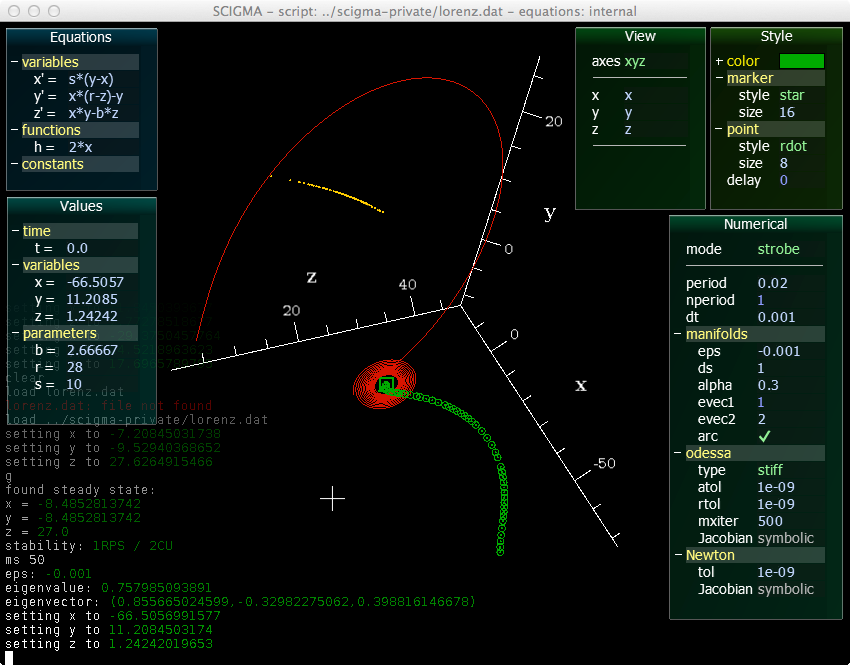
\includegraphics[width=\textwidth]{scigma.png}
\caption{Screenshot of a typical SCIGMA session}
\label{fig::screen}
\end{figure}
Figure \ref{fig::screen} shows SCIGMA's user interface. The largest part of the window is taken up by a diagram of the phase space and/or parameter space. On the sides, there are some panels that give you information about the current equation system, as well as all kinds of numerical and graphic settings. In the bottom left corner, there is a console at which you can enter equations and commands, as well as adjust and query the settings.\\
The first thing you have to do when working with SCIGMA is to let the program know which equations you want to look at. There are several ways to do that, which are all described in section \ref{sec::eq}. Once you have done that, you will be ready to produce some nice graphics. Most of SCIGMA's work is done by a handful of commands, namely
\begin{itemize}
\item{\HL{plot}, which plots orbits of maps and trajectories of differential equations,}
\item{\HL{guess}, which finds stationary states of trajectories and differential equations,}
\item{and \HL{mstable}/\HL{munstable}, which trace out invariant manifolds.}
\end{itemize}
These commands, together with some more bookkeeping and visual commands are described in section \ref{sec::comm}. Some other commands that you might find useful include
\begin{itemize}
\item{\HL{fit}, which scales the currently visible viewing area/volume such that objects fit onto the screen,}
\item{\HL{clear}, which deletes all objects in the graphics window,}
\item{and \HL{reset}, which, on top of clearing the graphics window, also deletes the current equation system.}
\end{itemize}
Of course there are a lot of options and settings that modify the behavior of SCIGMA's commands, the most important one being the \HL{mode} setting. \HL{mode} governs whether SCIGMA considers the system as a discrete map or as a differential equation, as well as whether it turns a set of differential equations into a stroboscopic map or Poincar\'e map. This and other settings are described in section \ref{sec::sett}.\\
Finally, section \ref{sec::mouse} describes how to navigate the viewing area (or viewing volume in three-dimensional projection) with the mouse, as well as how to interactively select objects and pick initial conditions for the numerical commands.

 \newpage\section{Specifying the equations}
 \label{sec::eq}
In SCIGMA, there are three ways of encoding equations, namely
\begin{itemize}
\item directly at the command line in the graphics window, or from a script file (best suited for the explorative investigation of smaller systems);
\item by specifying a set of equations in a Python script - Python is more expressive (e.g. loops and arrays
	are available), but you will have to specify the Jacobian yourself. 
\item	as a precompiled shared library (fastest, but less convenient than both of the above).
\end{itemize}
The next three sections describe all of these possibilities.\\\\
Before we dive into the specifics, let us discuss what all three approaches have in common: SCIGMA distinguishes between three types of user defined symbols in equations: \emph{variables, parameters} and \emph{functions}. The number of variables determines the dimension of the phase space for an ODE or a map. Parameters are values that are constant in time and may be used for bifurcation analysis (\emph{... coming soon ...}). Functions are quantities that depend on variables, or parameters, or both, which are not strictly necessary to describe the problem, but might be convenient as auxiliary functions or otherwise interesting. For illustration, look at these equations for an harmonic oscillator:
\begin{eqnarray}
\dot{x}&=&-y\nonumber\\ 
\dot{y}&=&\omega^2x\nonumber\\
\omega&=&\sqrt\frac{k}{m}
\label{example}
\end{eqnarray}
Here, $x$ and $y$ are variables, $k$ and $m$ are parameters and $\omega$ is a (constant) function.\\
Regardless of how the equations are specified, you can always set the value of a variable or a parameter like this
\C{x=1\\k=2}
at the SCIGMA console, or in the \T{Values} panel.

\subsection{At the SCIGMA console}
\label{sec::internaleq}
\subsubsection*{Variables}
To define a variable for an ODE system, all you have to do is provide its time derivative.\\
\T{x' = x-1}\\
defines a variable $x$ with $\dot{x}=x-1$. The initial condition / current value for $x$ is set like this:\\
\T{x = 0.5}\\
For an iterated map, the syntax to define a variable by providing the iterative equation, is the same:\\
\T{n' = n*2+1}\\
How your equations are interpreted depends on whether the \HL{mode} option of the program is set to \T{'ode', 'strobe' or 'Poincare'} (interpretation as ODE) or to \T{'map'} 
(interpretation as iterated map).
\subsubsection*{Parameters}
If you assign a value to a new symbol\\ 
\T{a = 2} ,\\
this defines a new parameter. Parameters are also created implicitly when a symbol appears in an expression
for the first time (see below).
\subsubsection*{Functions}
If the right hand side of your equation contains at least one symbol like \T{x}, \T{n}, and \T{a}, you create
a function rather than a parameter:\\
\T{xSquare = x**2}\\
Note that \T{xSquare} keeps track of the changes in \T{x} and updates itself accordingly, not only if
\T{x} changes its value, but even if it is completely redefined; as another example, consider this definition
for the time derivative of \T{y}:\\
\T{y' = x**2 + a**b}\\ 
Here, \T{a} is an already known parameter with value \T{2}, while \T{b} is implicitly initialized as a new parameter
with value \T{0}, which happens whenever you enter an equation with a symbol that is not yet defined. \T{x} is of course a variable since our first definition. For the moment, we have $\dot{y}=x^2+2^0$. Note that instead of the last line, you could also have written\\ 
\T{y' = xSquare + a**b} .\\ 
When you redefine a variable, parameter or function, this affects all other functions depending on it. For example after\\
\T{b = x+y} ,\\
the time derivative of \T{y} becomes $\dot{y}= x^2 + 2^{x+y}$. Because previous definitions are updated, the order in which you enter a set of equations does not matter; SCIGMA takes care that the equations remain consistent.\\
\subsubsection*{Evaluation operator}
If you do want to extract the current value of a function instead of the function itself, use the \$-operator:\\
\T{\$(a**2)}\\
prints out \T{4}, for example. Do NOT use this operator on the right hand of equations, this will erratically change the value
of the left hand side function.
\subsubsection*{Builtin mathematical functions}
There is a number of builtin mathematical operations understood by SCIGMA's parser that can be used in expressions. Please see table \ref{supp} for the full list. %Note that \T{abs}, \T{sign}, \T{step} and \T{mod} are non-differentiable and should be used judiciously on the right hand side of ODEs (there is no internal mechanism to deal with convergence problems caused by these functions).
\begin{table}
\centering
\begin{tabular}{l}
\textbf{supported mathematical operations}\\\hline
\T{+, -, *, /, **, sqrt, exp, ln, log10,}\\
\T{sin, cos, tan, asin, acos, atan, atan2,}\\
\T{sinh, cosh, tanh, asinh, acosh, atanh,}\\
\T{pow, sigmoid, pulse, abs, sign, step, mod} 
\end{tabular}
\caption{List of mathematical operations understood by SCIGMA's internal parser. \T{**} stands for exponentiation, as in FORTRAN or Python. \T{sigmoid} takes two arguments $x$ and $\beta$ and is defined as $s=(1+\exp(-x/\beta))^{-1}$; \T{pulse} also takes two arguments: $p=\exp(x/\beta)/(\beta\exp(x/\beta)+\beta)$, which is the derivative of the sigmoid function. Therefore, the area under the pulse is always equal to 1. The \T{step} function behaves like its GLSL equivalent, taking two parameters as well, where the second parameter is the position of the step. \T{mod} is equivalent to the C function \T{fmod}}
\label{supp}
\end{table}
%\subsubsection{Custom functions with arguments}
%Similar to mathematical functions like \T{sqrt}, you can define your own functions with arguments for later reuse:\\
%\T{f(x,y)=x**2+y**2}\\
%defines such a function. You can use \T{f} in other expressions and it will behave just like a normal function. When
%you call it with arguments\\
%\T{g=f(a,1)}\\ 
%though, the arguments will be inserted instead of the dummy arguments in \T{f}'s definition. As a result, the definition of \T{g}
%will be $g=a^2+1$.
\subsubsection*{Deleting variables, parameters and functions}
To delete all information pertaining to a symbol \T{x}, use\\
\T{!x} .\\
This deletes function definitions, map and ODE definitions and the symbol itself (unless there are symbols that depend on \T{x}; in this case, these have to be deleted first).
You can also do this\\
\T{!x'} ,\\ 
which takes the variable \T{x} out of the dynamical system, but keeps it available as parameter.
\begin{table}
\centering
\begin{tabular}{ll}
\textbf{command}&\textbf{effect}\\\hline
\T{x' = }\emph{value $\vert$ expression}&define variable \T{x}\\
\T{x = }\emph{expression}&define function \T{x}\\
%\T{x(}\emph{arglist}\T{) = }\emph{expression}&define user function \T{x} with arguments\\
\T{x = }\emph{value}&define parameter \T{x} / set value of variable \T{x}\\
\T{\$}\emph{expression}&replace expression by its current value\\
\T{!x}&delete symbol \T{x}\\
\T{!x'}&turn variable \T{x} into parameter \\
\end{tabular}
\caption{List of different command types understood by SCIGMA's internal parser. \emph{value} is any expression that evaluates to a constant, i.e. either a number, or a builtin function of just numbers like \T{sin(3.14)**2}.
\emph{expression} is any expression that depends on at least one other defined symbol like \T{sin(2*a)} or \T{f*g+1}.}
\label{comm}
\end{table}

\subsubsection*{Example}
Table \ref{comm} shows a summary of the available commands of SCIGMA's internal equation parser. With these commands, we are now ready to specify equations \eqref{example} from the beginning of this chapter:\\
\T{x'=-y}\\
\T{y'=omega**2*x}\\
\T{omega=sqrt(k/m)}\\
Before observing the dynamics, we must also assign sensible values to the parameters \T{k} and \T{m}, for example\\
\T{k=1}\\
\T{m=2}\\
Now the system can be used with SCIGMA. Note again that the order in which the five equations above are entered does not matter.\\\\ 
Instead of entering the equations step by step at runtime you can also collect them in a file and use the \HL{load} command. 
Either way, the equations will also be mirrored in the \T{Equations} panel, which can be used to modify the equations as well.

\subsection{In a Python script}
\label{sec::pythoneq}
You can load a set of equations from a Python file at runtime with the \HL{equations} command. SCIGMA scans this script for the following symbols:
\begin{description}
\item{\T{v\char`_names}} is a list of variable names:\\
\T{v\char`_names = ['x','y','z']}
\item{\T{v\char`_values}} is a list of initial values for the variables:\\
\T{v\char`_values = [0,0,0]}\\
If \T{v\char`_values} is defined, it must have the same length as \T{v\char`_names}. If it is not defined the variables are not initialized on equation loading.
\item{\T{p\char`_names}} is a list of parameter names:\\
\T{p\char`_names = ['a','b','c']}\\
If \T{p\char`_names} is not defined, SCIGMA assumes that there are no parameters.
\item{\T{p\char`_values}} is a list of initial values for the parameters:\\
\T{p\char`_values = [1,2,3]}\\
If \T{p\char`_values} is defined, it must have the same length as \T{p\char`_names}. If it is not defined the parameters are not initialized on equation loading.
\item{\T{f}} is a function defining the right hand side of the dynamical system. \T{f} can have one of these signatures:\\
\T{def f(x,xdot):}\\
\hphantom{mmm}\ldots\hspace{8em}\T{\# for autonomous systems without parameters}\\
\T{def f(x,p,xdot):}\\
\hphantom{mmm}\ldots\hspace{8em}\T{\# for autonomous systems with parameters}\\
\T{def f(t,x,xdot):}\\
\hphantom{mmm}\ldots\hspace{8em}\T{\# for non-autonomous systems without parameters}\\
\T{def f(t,x,p,xdot):}\\
\hphantom{mmm}\ldots\hspace{8em}\T{\# for non-autonomous systems with parameters}\\\\
SCIGMA decides on the type of system by looking at the number of arguments and the name of the first argument. Therefore, the first argument must always be \T{t} for non-autonomous systems. SCIGMA will pass the variables in the first argument (autonomous systems) or second argument (non-autonomous systems) and the parameters in the second or third argument. The right hand side must be written to the third (autonomous systems) or the fourth argument (non-autonomous systems). Note that \T{x}, \T{p} and \T{xdot} are raw pointers to memory, so you are responsible to not access them beyond their limits, which are given by the length of the \T{v\char`_names} and \T{p\char`_names} lists, respectively (the example below shows how the arguments are used). 
\item{\T{dfdx}} is a function defining the jacobian of the dynamical system. If \T{dfdx} is defined, it must have the same signature as \T{f}, for example\\
\T{def dfdx(x,jac):}\\
\hphantom{mmm}\ldots\hspace{8em}\T{\# for autonomous systems without parameters}\\\\
SCIGMA expects the Jacobian in column major ordering, i.e. if there are \T{N} variables, the first \T{N} entries of \T{jac} contain the partial derivatives of the right hand side with respect  to the first variable, the next \T{N} entries the partial derivatives with respect to the second variable and so on (compare also the example below). You do not need to provide zero elements of the Jacobian.
\item{\T{f\char`_names}} is a list of additional function names:\\
\T{f\char`_names = ['f,'g','h']}\\ 
If defined, these are some additional functions of interest which are computed and stored along with the variables. They are evaluated by calling 
\item{\T{func}}, which, must again have the same signature as \T{f}:\\
\T{def func(x,values):}\\
\hphantom{mmm}\ldots\hspace{8em}\T{\# for autonomous systems without parameters}\\\\
\T{func} must be defined if \T{f\char`_names} is defined and has at least one entry.	 
\end{description}

\subsubsection*{Example}
The Python script describing the example equations \eqref{example} would look like this:\\
\\
\T{import math}\\
\\
\T{v\char`_names=['x','y']}\\
\T{p\char`_names=['k','m']}\\
\T{p\char`_values=[1,2]}\\
\T{f\char`_names=['omega']}\\
\\
\T{def f(x,p,xdot):}\\
\hphantom{mmm}\T{xdot[0]=-x[1]}\\
\hphantom{mmm}\T{xdot[1]=p[0]/p[1]*x[0]}\\
\\
\T{def dfdx(x,p,jac):}\\
\hphantom{mmm}\T{jac[1]=p[0]/p[1]}\\
\hphantom{mmm}\T{jac[2]=-1}\\
\\
\T{def func(x,p,values):}\\
\hphantom{mmm}\T{values[0]=math.sqrt(p[0]/p[1])}\\
\\
Please note that you cannot use the additional functions inside the body of \T{f} or \T{dfdx} (this is because internally, \T{func} is not evaluated for every single call of \T{f} and \T{dfdx}). 
\subsection{In a Shared Library}
\ldots coming soon \ldots

\newpage\section{Commands}
\label{sec::comm}
In the list of commands below, mandatory arguments are written like \T{<this>}, optional arguments are written like \T{[this]}. If there are two or more distinct possibilities for an argument, they will be denoted \T{<like|this>} \T{[or|like|this]}. Most commands have abbreviations, which are given at the end of the description of the command.
\subsection{General}
\begin{description}
\cmd{equations}{['internal'|filename]}\\specifies the source of the dynamical equations. You can provide the equations either internally at the command line (this is the standard setting, to which you can return by giving \T{'internal'} as argument), or in a Python script file specified by \T{filename}. See sections \ref{sec::internaleq} and \ref{sec::pythoneq} for details on the format of internal equations and of the Python file, respectively. If neither \T{'internal'}, nor any \T{filename} is given as an argument, the command opens a file dialog. This command may be abbreviated by \T{eq}.
\cmd{load}{[filename]}\\loads and runs a the script file specified in \T{filename}. If \T{filename} is not given, the command opens a file dialog. This command may be abbreviated by \T{l}.
%\cmd{save}{<name> [filename]}\\
\cmd{select}{<name>}\\makes the object specified by \T{name} the currently selected object. This command may be abbreviated by \T{sel}.

\cmd{delete}{<name>}\\deletes the orbit, manifold or special point specified by \T{name} from memory, including all of the data. This command may be abbreviated by \T{del}.
\cmd{clear}{}\\
Deletes all orbits, manifolds and special points. This command may be abbreviated by \T{cl}.
\cmd{reset}{}\\
Deletes all orbits, manifolds and special points, deletes the current set of equations and resets the view to a two-dimensional plot of $x$ vs $y$ between $(-1,-1)$ and $(1,1)$. This command may be abbreviated by \T{res}.
\cmd{quit}{}\\closes the current window and frees the associated resources (i.e. makes them available to Python's
garbage collector). This command may be abbreviated by \T{q}.
\end{description}
\subsection{Numerical}
You will notice that some of the commands below come in two versions, namely with and without an appended asterisk (\T{*}). For these commands, the version with the asterisk shows \emph{all} iterates if \HL{nperiod} is not 1, while the command without the asterisk just shows the \emph{nperiod-th} iterates. 
\begin{description}
\cmd{plot}{[n] [name] / plot* [n] [name]}\\takes the current state as initial condition and plots \T{n} steps of the resulting orbit or trajectory. The orbit will be assigned \T{name} as identifier for further reference. If \T{n} is not given, only one step will be taken. A negative \T{n} will reverse the direction of the iteration/integration. If \T{name} is not given, a unique name of the form \T{'trN'} will be generated.\\
The behavior of this command depends on the current setting of the \HL{mode} option:\\
If \HL{mode} is \T{map}, the program iterates the map and plots every \HL{nperiod}-th point.\\
If \HL{mode} is \T{ode}, the program integrates the differential equations for \T{n} time steps \HL{dt} and plots the trajectory.\\
If \HL{mode} is \T{strobe}, 
the program will plot every \HL{nperiod}-th point of the stroboscopic map of the differential equations with a time interval \HL{period} (this is effectively the same behavior as for \T{ode}, with \HL{period}$\times$\HL{nperiod} as time step instead of \HL{dt}).\\
If \HL{mode} is \T{Poincare}, the program constructs a Poincare map for the intersection of the \HL{secvar}$=$\HL{secval} plane, iterates it and plots every \HL{nperiod}-th point. \HL{maxtime} determines how far the program should integrate before giving up on finding an intersection. \HL{secdir} determines whether the value of \HL{secvar} should be increasing or decreasing at the intersection.\\ 
The appearance of the resulting trajectory in depends on the current values of \HL{color}, \HL{marker.style}, \HL{marker.size}, \HL{point.style}, \HL{point.size} and \HL{delay}. This command may be abbreviated by \T{p / p*}.
\cmd{guess}{[name] / guess* [name]}\\takes the current state as starting point and tries to find a stationary state or the current map or ode by Newton iteration. If a stationary state is found, it will be assigned \T{name} as identifier for further reference. If \T{name} is not given, a unique name of the form 
\T{'fpN'} ('fixed point', for differential equations) or \T{'ppN'} ('periodic point', for maps) will be generated. If \HL{mode} is not \T{ode}, the program will look for a stationary state of the \HL{nperiod}-th iterate of the map. Stationary states of differential equations will be marked with a circle, if they are unstable, and with circles with a dot in the center, if they are stable. Stationary states of maps will be marked with an empty square, if they are unstable, and with a square with a dot in the center, if they are stable. The further appearance depends on the current values of \HL{color}, and \HL{marker.size}. This command may be abbreviated by \T{g / g*}.
\cmd{evals}{[name]}\\
prints the eigenvalues of the object specified by \T{name}. If \T{name} is not given, the currently selected object is used.  
\cmd{evecs}{[name]}\\
prints the eigenvectors of the object specified by \T{name}. If \T{name} is not given, the currently selected object is used.  
\cmd{mstable}{[n] [origin] [name] / mstable* [n] [origin] [name]}\\takes a stationary state (the 'origin') previously found with \HL{guess} and plots \T{n} steps of the 1-dimensional unstable manifold of the origin along an unstable eigenvector, which is determined by the value of \HL{evec1}.  \T{name} will be assigned to the manifold as identifier for further reference. If \T{n} is not given, just the initial segment is created. If \T{origin} is not given, the currently selected object is used. If \T{name} is not given, a unique name of the form \T{'mfN'} will be generated. If \HL{mode} is \T{ode}, one step will correspond to an integration of $\pm$\HL{dt}. Otherwise, the manifold for the \HL{nperiod}-th iterate of the map will be constructed, with an arc length step of (roughly) \HL{ds}. The accuracy of the manifold stepping algorithm for maps can be adjusted with \HL{alpha}. The appearance of the manifold depends on the current values of \HL{color}, \HL{marker.style}, \HL{marker.size}, \HL{point.style}, \HL{point.size} and \HL{delay}. This command may be abbreviated by \T{ms / ms*}.
\cmd{munstable}{[n] [origin] [name] / munstable* [n] [origin] [name]}\\
works analog to \T{mstable}. This command may be abbreviated by \T{mu / mu*}.
%\cmd{m2unstable}{[n] [origin] [name]}\\
%This command may be abbreviated by \T{mu}.
%\cmd{m2stable}{[n] [origin] [name]}\\
%This command may be abbreviated by \T{ms}.
\cmd{rtime}{[name]}\\
If \T{name} denotes an orbit or stationary state of a stroboscopic map or Poincare map, this prints the return time. If \T{name} is not given, \T{rtime} prints the return time of the currently selected object. This command may be abbreviated by \T{rt}.
\cmd{circle}{<diameter> [n]}\\
takes the current position as center and places \T{n} initial conditions equally spaced on the circle with the specified diameter. \T{diameter} is given in units of the currently visible portion of phase space. If \T{n} is not given, 100 is used. This command may be abbreviated by \T{cir}.
\end{description}
\subsection{View and style}
\begin{description}
\cmd{hide}{<name>}\\hides the orbit, manifold or special point specified by \T{name} if it is currently on display, but keeps it in memory.
\cmd{show}{<name>}\\displays the orbit, manifold or special point specified by \T{name} if it is currently hidden.
\cmd{2d}{}\\changes to two-dimensional projection.
\cmd{3d}{}\\changes to three-dimensional projection.
\cmd{xrange}{<min> <max>}\\adjusts the range of the x dimension. \T{min} must be smaller than \T{max}.
\cmd{yrange}{<min> <max>}\\adjusts the range of the y dimension. \T{min} must be smaller than \T{max}.
\cmd{zrange}{<min> <max>}\\adjusts the range of the z dimension. \T{min} must be smaller than \T{max}.
\cmd{crange}{<min> <max>}\\adjusts the range of the color dimension. \T{min} must be smaller than \T{max}.
\cmd{fit}{}\\
adjusts the viewing volume to include all visible objects. This command may be abbreviated by \T{f}.
\end{description}

\newpage\section{Settings}
\label{sec::sett}
Settings can be changed on the command line with the syntax given below. If only the name of an option is entered, SCIGMA prints its value on the console. Instead of using the command line, you can also access all settings using the \T{Numerical}, \T{View} and \T{Style} panels.
\subsection{Numerical}
\begin{description}
\opt{mode}{<'m[ap]'|'o[de]'|'s[trobe]'|'P[oincare]'>}\\ 
specifies which type of dynamical problem is investigated. If \T{mode} is set to \T{map}, the equations are interpreted as a discrete map, otherwise they are interpreted as system of ordinary differential equations. The behavior of most numerical commands, as well as the availability and relevance of other numerical options depends on the value of \T{mode}. The default value is \T{ode}.
\opt{period}{<value>}\\
sets the return time for stroboscopic maps (\HL{mode} is \T{strobe}). If \HL{equations} are internal, \T{value} can be any expression that  evaluates to a constant ($value$ in the sense of table \ref{comm}), for example \T{\$(2*pi/omega)}. If \HL{equations} are not internal, \T{value} must either be a number, or the value of a symbol defined in the equation system, prefixed with the \$-operator, for example \T{\$T}. The default value is \T{1.0}. 
\opt{nperiod}{<value>}\\
sets the number of periods for the iteration of maps. \T{value} must be an integer. All algorithms (basically \HL{plot}, \HL{guess} and the manifold commands) acting on maps (regular, stroboscopic and Poincar\'e), will use the \T{nperiod}-th iterate of the map. The default value is \T{1}.
\opt{dt}{<value>}\\
sets the time step for the integrator. This is relevant for all settings of \HL{mode} except the \T{map} setting. \T{dt} must be positive real number. If you want to \HL{plot} backwards in time, use a negative step size. The default value is \T{0.001}. 
\opt{secvar}{<varname>}\\
sets the variable of the Poincar\'e section. \T{varname} must be a variable that is part of the current equation system. The default value is \T{'x'}.
\opt{secval}{<value>}\\ 
sets the variable value of the Poincar\'e section. \T{value} must be a positive real number, the default value is \T{0.0}.
\opt{secdir}{<'+'|'-'>}\\
sets the direction in which crossings of Poincar\'e section are detected. If \T{'+'}, crossings with increasing value of \HL{secvar} are detected, if \T{'-'}, crossings with decreasing value of \HL{secvar} are detected. The default value is \T{'+'}.
\opt{maxtime}{<value>}\\ 
determines, until which value of $t$ SCIGMA integrates to find a section of the Poincar\'e plane, before throwing the towel. \T{value} must be a positive real number, the default value is \T{100.0}.
\opt{eps}{<value>}\\
sets the distance of the initial segment of invariant manifolds from a stationary state. \T{value} must be a non-zero real number. By changing the sign, you can plot the two parts of one-dimensional manifolds. The default value is \T{0.0001}. 
\opt{ds}{<value>}\\
sets the arc length step for invariant manifolds of maps (not used if \HL{mode} is \T{ode}). \T{value} must be a positive real number, the default is \T{0.01}.
\opt{alpha}{<value>}\\
sets the maximum accepted angle for consecutive line segments on invariant manifolds of maps (not used if \HL{mode} is \T{ode}). \T{value} must be a positive angle in rad. Internally, SCIGMA uses an adapted step size algorithm to approximate invariant manifolds of maps. If two consecutive line segments have an angle of more than \T{alpha}, the internal step size is reduced. The default value is \T{0.3}.
\opt{evec1}{<value>}\\
sets the first eigenvector that is used when computing invariant manifolds. \T{value} must be a positive integer, no larger then the number of dimensions in the current equations system. The eigenvalues of any stationary state are sorted according to stability (i.e. with ascending real value for ODEs, with ascending modulus for maps). For a stable (unstable) manifold the \T{evec1}-th most stable (unstable) eigenvalue is selected. The default value is \T{1}, for the selection of the most stable (unstable) eigenvalue.
%\opt{evec2}{<value>}\\
%\opt{arc}{<'true'|'false'>}\\
\opt{Newton.tol}{<value>}\\ 
sets the tolerance of the Newton-Raphson algorithm that is used for finding stationary states, and also to converge onto Poincar\'e planes. \T{value} must be a positive real number, the default is \T{1e-9}.
\opt{atol}{<value>}\\
sets the absolute tolerance of the ODESSA integration algorithm. \T{value} must be a positive real number, the default is \T{1e-9}.
\opt{rtol}{<value>}\\
sets the relative tolerance of the ODESSA integration algorithm. \T{value} must be a positive real number, the default is \T{1e-9}.
\opt{type}{<'non-stiff'|'stiff'>}
sets whether the ODESSA integrator should use an algorithm for non-stiff or stiff equations. The default value is \T{'stiff'}.
\opt{mxiter}{<value>}\\
sets the number of internal steps before the ODESSA integrator bails out if it does not converge. \T{value} must be a positive integer, the default is \T{500}.
switches between
\end{description}
\subsection{View and style}
\begin{description}
\opt{axes}{<'xy','xyz','xyc','xyzc'>}\\
sets the whether the current view is 2D (\T{'xy'}), 2D with a color map (\T{'xyc'}), 3D (\T{'xyz'}) or 3D with a color map (\T{'xyzc'}). The default is \T{'xy'}.
\opt{color}{<name|r g b [a]|index>}\\
sets the drawing color for new objects. There are three ways of specifying the color:
\begin{itemize}
\item{using the name, e.g. \T{color green}; available names are \T{'red'}, \T{'green'}, \T{'blue'}, \T{'yellow'}, \T{'pink'}, \T{'lime'}, \T{'azure'}, \T{'orange'}, \T{'brown'}, \T{'forest'}, \T{'navy'}, \T{'teal'}, \T{'rose'}, \T{'aqua'}, \T{'sky'}, \T{'beige'}, \T{'black'}, \T{'dark\char`_gray'}, \T{'gray'}, \T{'light\char`_gray'}, \T{'white'}, \T{'cyan'} and \T{'magenta'}.}
\item{using rgb (and potentially alpha) values, e.g. \T{color 1 0 1 [1]} for magenta; all values must be real numbers between \T{0.0} and \T{1.0}, alpha values are optional.}
\item{using  an index, e.g. \T{color 6} for orange; the index must be an integer from \T{0}-\T{22} which points into the list of colors given above.}
\end{itemize}
The default value is \T{color red} = \T{color 0.75 0 0} = \T{color 0}.
\opt{delay}{<value>}\\
sets the artificial plotting delay. \T{value} must be a non-negative real number. If not zero, SCIGMA waits for \T{delay} seconds before plotting the next step of an orbit or manifold that is currently computed. This can be used to better observe the evolution of a state in phase space over time. Also, if \HL{marker.style} is not \T{none}, the current point of the orbit or trajectory is marked with a small graphic, which is easier to track. Plotting with delay only works correctly, however, if a single step can be computed faster than \T{delay}, otherwise the speed of the integration/manifold plotting algorithm determines how fast things are plotted. The default value is \T{0.0}.  
\opt{marker.style}{}\\
sets the marker style for plotting with \HL{delay}. Possible values are \T{'dot'}, \T{'plus'}, \T{'ring'}, \T{'rdot'}, \T{'rplus'}, \T{'rcross'}, \T{'quad'}, \T{'qdot'}, \T{'qplus'}, \T{'qcross'}, \T{'hash'}, \T{'star'} and \T{'none'}. The default value is \T{'star'}. 
\opt{marker.size}{}\\
sets the marker size for plotting with \HL{delay} and for marking stationary states. \T{value} must be a positive real number (values larger than \T{64.0} may not be supported by the OpenGL implementation). The default value is \T{16.0}.
\opt{point.style}{}\\
sets the point style for plotting orbits, trajectories and one-dimensional manifolds. Possible values are \T{'dot'}, \T{'plus'}, \T{'ring'}, \T{'rdot'}, \T{'rplus'}, \T{'rcross'}, \T{'quad'}, \T{'qdot'}, \T{'qplus'}, \T{'qcross'}, \T{'hash'}, \T{'star'} and \T{'none'}. The default value is \T{'none'} (in this case, the points are connected by line segments).
\opt{point.size}{}\\ 
sets the point size for plotting orbits, trajectories and one-dimensional manifolds.  \T{value} must be a positive real number (values larger than \T{64.0} may not be supported by the OpenGL implementation). The default value is \T{8.0}.
\end{description}
 \newpage\section{Mouse navigation}
\label{sec::mouse}
\subsection{Rotating}
If the current projection is three-dimensional (see \HL{axes} option and the \HL{2d}/\HL{3d} commands), you can rotate the viewing volume by pressing the left mouse button somewhere over an empty region of the graphics window and dragging the mouse.
\subsection{Shifting}
You can shift the viewing area/volume along the horizontal and vertical axes of the screen by pressing the left mouse button somewhere over an empty region of the graphics window and dragging the mouse while also pressing the shift key. Alternatively, if you let the cursor hover over one of the axes, such that it is highlighted, you can shift along this axes by pressing the left mouse button and dragging the mouse.
\subsection{Zooming}
You can change the scale of the viewing area/volume by scrolling with the mouse wheel, while the cursor is over an empty region of the graphics window. This zooms in and out equally for all axes. Alternatively, if you let the cursor hover over one of the axes, such that it is highlighted, you can scale just this axis by scrolling with the mouse wheel.
\subsection{Picking points}
If the projection is two-dimensional, double clicking somewhere in the graphics window will make the two coordinates of this point current. You will also see a white crosshair shape marking the point. In three-dimensional projection, the first double click will define a line of sight. If you rotate the viewing volume, you will see the line of sight as it runs through the viewing volume. On it, there is a white crosshair shape that follows the movement of the mouse. If you are satisfied with the position of the crosshair, double click again, and the three coordinates of the point will be made current. Also, the point is marked by the crosshair.\\
Both in two and three dimensions you can pick more than one point. To do so, press the control key while performing the steps above multiple times. As a result, you will get a number of crosshair shapes, marking your set of newly picked initial conditions. Commands like \HL{plot} will now act simultaneously on all of these.
\subsection{Picking objects}
Whenever the mouse hovers over an object like a trajectory in the graphics window, the object is highlighted. If you now double click, this will select the object under the cursor as current object. The current object is used by commands like \HL{munstable}, if no object is explicitly given as an argument. Also, the coordinates of the object (in case of orbits and trajectories: the last point) are made current.
\newpage\section{The Python layer}
\ldots coming soon \ldots
\section{The C++ layer}
\ldots coming soon \ldots

\printindex*

\end{document}
